\section{Theorie}
\label{sec:theorie}
Mittels eines Operationsverstärkers lässt sich eine Ausgangsspannung $U_a$ erzeugen, welche
proportional zur Differenz zweier angelegter Eingangsspannungen ist.
Der Operationsverstärker ist ein Bauteil welches im Allgemeinen über zwei Spannungseingänge, zwei Anschlüsse
für die Betriebsspannung $U_B$ und einen Ausgang
verfügt. In Schaltskizzen wird
das in \autoref{fig:opskizze} gezeigte Symbol für den Operationsverstärker verwendet.
\begin{figure}[H]
    \centering
    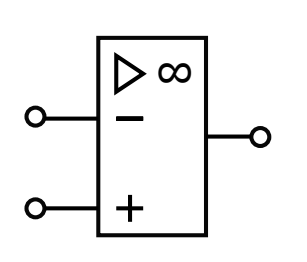
\includegraphics[width=0.2\textwidth]{op.png}
    \caption{Schaltzeichen des Operationsverstärkers \cite{anleitung} nach der Norm DIN-EN-6067.}
    \label{fig:opskizze}
\end{figure}
Dabei beschreibt
\textbf{+} die Eingangsspannung, die in Phase geschaltet ist und daher auch als nicht-invertierender
Eingang beschrieben wird, während \textbf{-} der gegenphasige oder invertierende Eingang
zur Ausgangsspannung ist. Die Ausgangsspannung ist dadurch definiert als
\begin{equation*}
    U_a = V \cdot  (U_+ - U_-),
\end{equation*}
wobei $U_{\pm}$ die angelegte Spannung an den jeweiligen Eingängen und $V$ die Leerlaufverstärkung ist.
Die Ausgangsspannung ist dabei durch die Betriebsspannung über
\begin{equation*}
    - U_B < U_a < U_B
\end{equation*}
begrenzt.

Zur theoretischen Beschreibung eines Operationsverstärkers werden in der Regel idealisierende
Annahmen getroffen. Im idealen Operationsverstärker ist sowohl die Verstärkung, als auch
der Eingangswiderstand unendlich groß ($V = \infty$ und $R_E = \infty$),
während es keinen Ausgansgwiderstand gibt ($R_A = 0$). \\
In einem realen Operationsverstärker sind diese Idealisierungen nicht zu erreichen, sodass im Bauteil
Leerlaufverstärkung und Eingangswiderstand nur möglichst groß und der Ausgansgwiderstand möglichst
klein sind. Da die Theorie Operationsverstärker mit diesen Idealisierungen beschreibt,
kommen in der Realität noch Korrekturen, wie Offsetstrom und Offsetspannung, welche
daher stammen, dass die Eingangsströme bei realen Operationsverstärkern endlich sind oder
der Gleichtaktverstärkung, welche ein Maß für die Verzerrung innerhalb des Bauteils ist, hinzu.

\subsection{Invertierender Linearverstärker}
Die Schaltskizze eines invertierenden Linearverstärkers ist in \autoref{fig:lin} zu sehen. Er wird
verwendet um ein invertiertes, verstärktes Signal bezüglich der Eingangsspannung $U_e$ zu erzeugen.
\begin{figure}[H]
    \centering
    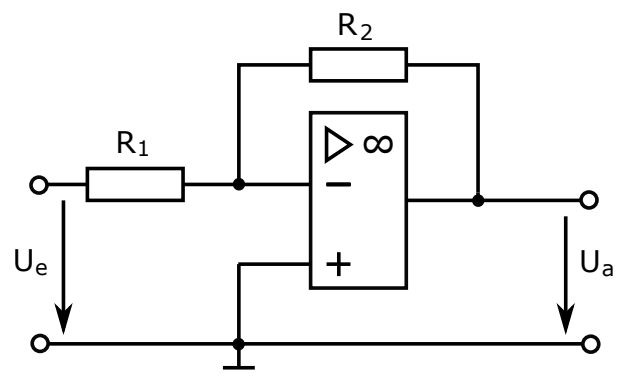
\includegraphics[width=0.4\textwidth]{linear.png}
    \caption{Schaltskizze des invertierenden Linearverstärkers \cite{anleitung}.}
    \label{fig:lin}
\end{figure}
Bei diesem Aufbau wird der invertierende Eingang über zwei Widerstände rückgekoppelt,
sodass ein Teil der
Ausgangsspannung an den invertierenden Eingang zurückgegeben wird. An dieser Anschlussstelle
ist die Spannung gering, sodass sich über die Kirchhoff'schen Regeln die Gleichung
\begin{equation*}
    \frac{U_e}{R_1} + \frac{U_a}{R_2} = 0
\end{equation*}
bestimmen lässt. Die Bezeichnungen stimmen dabei mit denen aus \autoref{fig:lin} überein.
Die ideale Leerlaufverstärkung $V'$ ist durch
\begin{equation}
    \label{eqn:verhaeltnis}
    V' = \frac{U_a}{U_e} = - \frac{R_2}{R_1}
\end{equation}
gegeben. Im Idealfall ist die Leerlaufverstärkung also nur durch das Verhältnis der Widerstände
gegeben, da die Spannung $U_+$ am nicht-invertierenden Eingang verschwindet.
An der Anschlussstelle (As) ergibt sich für einen unbelasteten Spannungsteiler ($I_\text{As}=0$)
\begin{equation*}
    U_\text{AS} = - \frac{U_a}{V}
\end{equation*}
mit der realen Verstärkung $V$ und daher
\begin{equation*}
   V =  \frac{U_\text{AS} - U_1}{U_a - U_e} = \frac{R_1}{R_1 + R_2}.
\end{equation*}
Über \autoref{eqn:verhaeltnis} ergibt sich
\begin{equation*}
    \frac{1}{V'} \approx \frac{1}{V} + \frac{R_1}{R_2}.
\end{equation*}
Durch die Rückkopplung können Schwankungen von $V$ sehr gut abgefangen werden, sodass
$V'$ durch diese Schwankungen kaum betroffen ist. Die Gegenkopplung erhöht somit die Stabilität
der Verstärkungsschaltung.
Die Bandbreite $B$ gibt den Frequenzbereich konstanter Verstärkung an.
Die Verstärkung $V$ und die Bandbreite $B$, hängen dabei über die Beziehung
\begin{equation*}
    V \cdot B = \text{const.}
\end{equation*}
zusammen.
\subsection{Umkehr-Integrator}
Die Schaltskizze des Umkehrintegrators ist in \autoref{fig:umkehrint} zu sehen.
\begin{figure}[H]
    \centering
    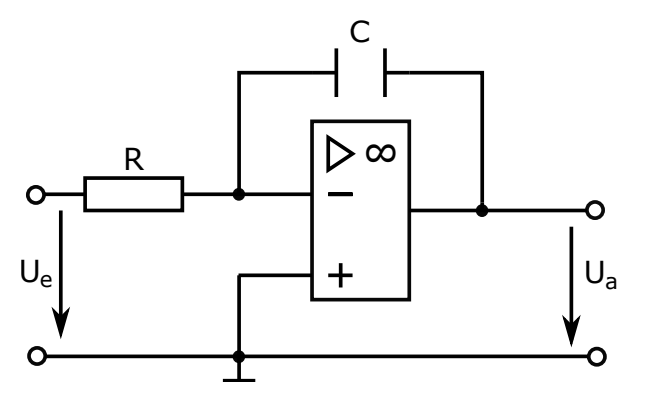
\includegraphics[width=0.4\textwidth]{integrator.png}
    \caption{Schaltskizze des Umkehr-Integrators \cite{anleitung}.}
    \label{fig:umkehrint}
\end{figure}
Im Vergleich zur vorherigen Schaltung in \autoref{fig:lin} wird der Widerstand $R_2$ durch einen
Kondensator $C$ ersetzt.
Dadurch wird die Eingangsspannung $U_e$ über die Zeit integriert zu
\begin{equation*}
    \int I_C \; \symup{d} t = C \cdot U_a.
\end{equation*}
Über die Knotenregel, sowie dem Zusammenhang $U = R \cdot I$ ergibt sich für die Ausgangsspannung
\begin{equation*}
    U_a = - \frac{1}{RC} \int U_e (t) \symup{d} t
\end{equation*}
und damit für ein sinusförmiges Eingangssignal $U_e = U_0 \sin(\omega t)$
\begin{equation*}
    U_a = \frac{U_0}{\omega R C} \cos(\omega t).
\end{equation*}
Es ergibt sich also ein antiproportionaler Zusammenhang zwischen der Ausgangsspannung $U_a$
und der Frequenz $\omega$. Allgemein können auch alle anderen Signale integriert werden.
Bei Unstetigkeiten kann es dabei allerdings zum sogenannten Gibb'schen Phänomen kommen,
also zu Überschwingungen an den Unstetigkeiten.

\subsection{Umkehr-Differentiator}
Werden nun Kondensator und Widerstand aus der vorherigen Schaltung vertauscht, ergibt sich
ein Umkehr-Differentiator. Die Schaltung dazu ist in \autoref{fig:umkehrdiff}
dargestellt.
\begin{figure}[H]
    \centering
    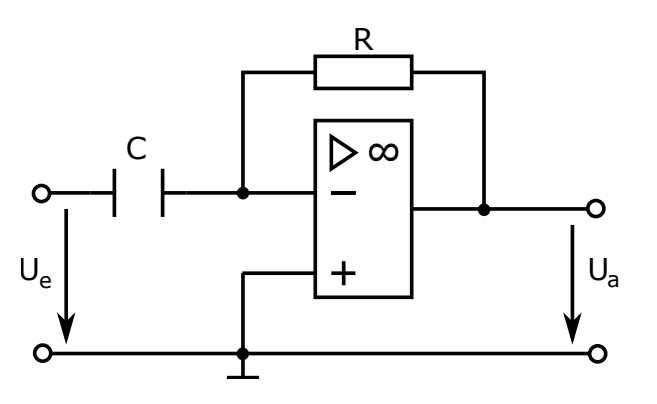
\includegraphics[width=0.4\textwidth]{diff.png}
    \caption{Schaltskizze des Umkehr-Differenzierers \cite{anleitung}.}
    \label{fig:umkehrdiff}
\end{figure}
Mit der Knotenregel ergibt sich
\begin{equation*}
    C \frac{\symup{d} U_e(t)}{\symup{d} t} + \frac{U_a(t)}{R} = 0
\end{equation*}
und durch Differentiation und Umstellen
\begin{equation*}
    U_a = - R C \frac{\symup{d}U_e}{\symup{d} t}
\end{equation*}
und somit für ein sinusförmiges Signal
\begin{equation*}
    U_a = - \omega R C U_0 \cos(\omega t).
\end{equation*}
Die Ausgangsspannung ist also direkt proportional zur Frequenz des Eingangssignals.

\subsection{Nicht-invertierender Schmitt-Trigger}
Um den Schmitt-Trigger zu bauen, wie in \autoref{fig:schmitt} zu sehen, wird eine sogenannte
Mitkopplung auf den nicht-invertierenden Eingang über einen Widerstand gelegt, womit der
Operationsverstärker die Eigenschaft eines Schalters erhält.
\begin{figure}[H]
    \centering
    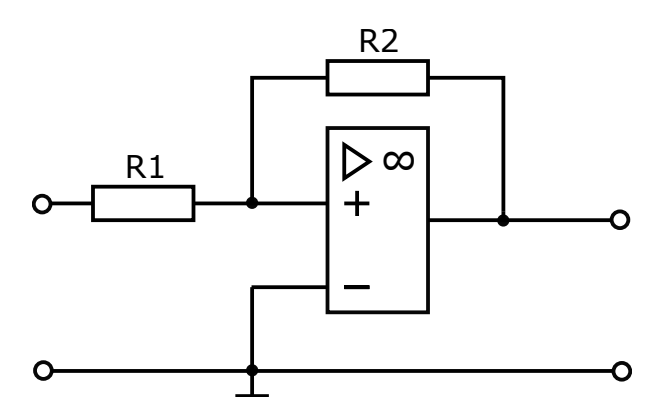
\includegraphics[width=0.4\textwidth]{schmitt.png}
    \caption{Schaltskizze des nicht-invertierenden Schmitt-Triggers \cite{anleitung}.}
    \label{fig:schmitt}
\end{figure}
Dies bedeutet, dass der Operationsverstärker
bei einem Schwellwert $U_{S_{\pm}}$ schlagartig den Sättigungswert $\pm U_B$ annimmt.
Die Schwellspannung ist dabei abhängig davon ob vor Veränderung des Eingangs eine
positive oder negative Ausgangsspannung vorliegt.
Die Schwellspannungen sind
\begin{equation*}
    U_{S_{\pm}} = U_{\pm} \frac{R_1}{R_2}.
\end{equation*}

\subsection{Signalgenerator}
Durch Kombination von Schmitt-Trigger (\autoref{fig:schmitt}) und Integrator (\autoref{fig:umkehrint})
ist es möglich einen Signalgenerator zu bauen, wie er in \autoref{fig:signal} skizziert ist.
Der Schmitt-Trigger liefert eine konstante Spannung $U_B$ bis der Schwellwert $U_{S_{-}}$
unterschritten wird. Bei Verwenden eines sinusförmigen Signals, welches die Schwellspannungen überschreitet,
gibt der Schmitt-Trigger
ein Rechtecksignal aus. Der Integrator integriert das Rechtecksignal zu einer Dreiecksspannung, die dort
ebenfalls abgegriffen werden kann. Die Frequenz der Schwingung hat den Theoriewert\cite{anleitung}
\begin{equation}
    \nu_{\text{Dreieck}} = \frac{R_2}{4 C R_1 R_3}.
    \label{eq:dreieck}
\end{equation}
\begin{figure}[H]
    \centering
    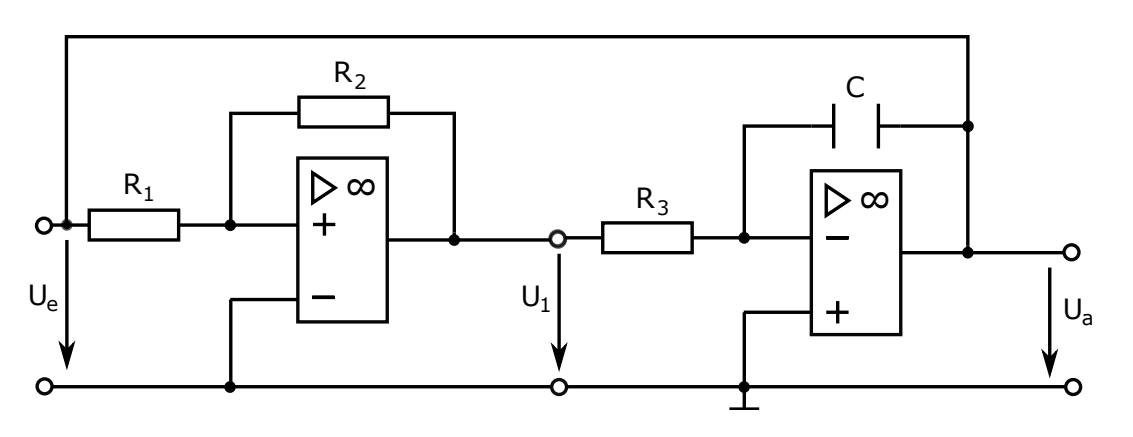
\includegraphics[width=0.67\textwidth]{signalgenerator.png}
    \caption{Schaltskizze des Signalgenerators \cite{anleitung}.}
    \label{fig:signal}
\end{figure}

\subsection{Variierende Amplituden}
Durch das Hintereinanderschalten von zwei Integratoren und einem invertierenden Linearverstärker
kann eine gedämpfte harmonische Schwingung erzeugt werden. Die Schaltskizze ist in
\autoref{fig:amplituden} dargestellt.
\begin{figure}[H]
    \centering
    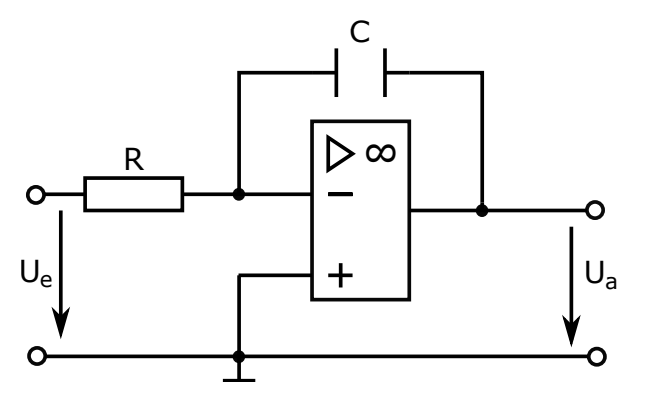
\includegraphics[width=0.4\textwidth]{integrator.png}
    \caption{Schaltskizze für variierende Sinusamplituden \cite{anleitung}.}
    \label{fig:amplituden}
\end{figure}
Diese Schwingung lässt sich durch die Differentialgleichung der Ausgangsspannung $U_a$ als Funktion der Zeit $t$
\begin{equation*}
    \frac{\symup{d^2} U_a}{\symup{d} t^2} - \frac{\eta}{10 R C} \frac{\symup{d} U_a}{\symup{d} t} + \frac{1}{R^2 C^2} U_a = 0
\end{equation*}
beschreiben, dessen Lösung
\begin{equation*}
    U_a (t) = U_0 \exp \left( \frac{\eta}{10 R C} \right) \sin \left(\frac{t}{R C} \right)
\end{equation*}
ist.
Dabei beschreibt $ -1 \leq \eta \leq 1 $ eine durch ein Potentiometer einstellbare Dämpfung.
Die Schwingungsdauer $T$ ist gegeben durch das sinus-Argument der Lösung der Differentialgleichung zu
\begin{equation*}
    T = 2 \pi R C
\end{equation*}
und die Abklingdauer beziehungsweise Zunahmedauer ist gegeben durch den Exponentialterm zu
\begin{equation*}
    \tau = \frac{20 R C}{\vert \eta \vert}.
\end{equation*}
